\chapter{Resultados}
\label{chap:results}

Este capítulo apresenta a avaliação da infraestrutura de comunicação desenvolvida, com foco no estabelecimento de conectividade e na transferência de dados entre aplicações TCP associadas a \textit{gateways} situados em redes distintas. A avaliação busca verificar o funcionamento da integração entre QUIC e ICE, considerando os caminhos de comunicação selecionados, a preservação dos dados transportados e o comportamento da solução durante a manutenção e o encerramento das conexões, como proposto pelos cenários de teste do Capítulo~\ref{chap:implementation}.

Inicialmente, são descritos o ambiente experimental, os cenários de teste e os critérios utilizados para analisar os resultados. Em seguida, são apresentados os testes de funcionamento e as medições de desempenho, relacionando as observações aos objetivos do trabalho. A discussão limita-se às configurações e às condições efetivamente avaliadas, sem pressupor a validação de um sistema IoT completo.

Além disso, são propostas na Seção~\ref{sec:another_connection_approaches} outras possíveis abordagens a serem comparadas apenas em nível lógico, o que implica que essa comparação não foi feita a partir de cenários de teste, mas apenas a partir dos conhecimentos previamente descritos nos Capítulos~\ref{chap:background} e~\ref{chap:quic}.

\section{Objetivo e metodologia da avaliação}

A avaliação tem como objetivo verificar se a infraestrutura desenvolvida permite estabelecer comunicação e transportar corretamente dados entre aplicações TCP associadas a \textit{gateways} situados em redes distintas. Os testes abrangem a integração entre QUIC e ICE, considerando o estabelecimento da conexão, a transferência bidirecional de dados, a manutenção da sessão e o encerramento dos recursos utilizados.

A metodologia compreende testes funcionais e medições de desempenho. Os testes funcionais verificam o comportamento da solução em cenários com comunicação direta e com retransmissão por TURN. A correção da transferência é verificada pela comparação entre os dados enviados e recebidos pelas aplicações. Nos testes de manutenção, são intercalados períodos de transferência e de inatividade para observar a continuidade da comunicação na mesma sessão.

Uma execução funcional é considerada bem-sucedida quando o caminho de comunicação esperado é selecionado, a conexão é estabelecida dentro do prazo definido, os dados são transferidos sem divergências e o encerramento ocorre sem erros. 

As medições de desempenho consideram o tempo de estabelecimento da comunicação, o tempo de resposta das aplicações e a vazão útil. Cada intervalo de medição é delimitado por eventos explícitos da execução, distinguindo o estabelecimento completo da infraestrutura do \textit{handshake} QUIC isolado. Os parâmetros de carga, a quantidade de repetições e os procedimentos de coleta são definidos para cada experimento e mantidos equivalentes nos cenários comparados.

Os testes utilizam dados sintéticos para avaliar o transporte entre os \textit{gateways}. A avaliação não inclui aquisição de dados por sensores físicos ou validação de requisitos de uma aplicação IoT específica. As conclusões são restritas aos ambientes, às configurações e às cargas efetivamente utilizados.

\section{Ambiente experimental e cenários com PatchBay}
\label{sec:experimental_patchbay}

Os experimentos utilizam as topologias descritas nas Seções~\ref{sec:basic_topology_network_namespaces}  e~\ref{sec:ice_topology_network_namespaces}, executadas com o PatchBay sobre \textit{Linux Network Namespaces}. Esta seção registra a configuração do ambiente e as diferenças entre os cenários de teste. A organização das interfaces de transporte e dos protocolos é apresentada no Capítulo~\ref{chap:implementation}.

\subsection{Plataforma e serviços auxiliares}

Os testes foram executados em ambientes com Ubuntu 24.04 LTS e Rocky Linux 8.10. A Tabela~\ref{tab:experimental_software} apresenta as versões das dependências utilizadas.

\begin{table}[htbp]
    \centering
    \label{tab:experimental_software}
    \begin{tabular}{@{}p{0.22\textwidth}p{0.14\textwidth}p{\dimexpr0.64\textwidth-4\tabcolsep\relax}@{}}
        \toprule
        \textbf{Componente} & \textbf{Versão} & \textbf{Função} \\
        \midrule
        OpenSSL & 4.1.0 &
        Implementação QUIC e proteção criptográfica. \\
        \texttt{libnice} & 0.1.21 &
        Coleta de candidatos, negociação ICE e transporte
        direto ou via TURN. \\
        \texttt{coturn} & 4.6.3 &
        Fornecimento dos serviços STUN e TURN. \\
        PatchBay & 0.7.0 &
        Criação e configuração da rede de testes. \\
        \bottomrule
    \end{tabular}
    \caption{Software utilizado no ambiente experimental.}
\end{table}

Os serviços auxiliares executam no nó ISP, conforme a topologia ICE apresentada na Seção~\ref{sec:ice_topology}. Sua configuração é resumida na Tabela~\ref{tab:experimental_services}.

\begin{table}[htbp]
    \centering
    \label{tab:experimental_services}
    \begin{tabular}{@{}p{0.28\textwidth}p{\dimexpr0.72\textwidth-2\tabcolsep\relax}@{}}
        \toprule
        \textbf{Elemento} & \textbf{Configuração} \\
        \midrule
        STUN/TURN &
        Comunicação por UDP, na porta 3478.
        O adaptador utiliza
        \texttt{NICE\_RELAY\_TYPE\_TURN\_UDP};
        TCP, TLS e DTLS estão desabilitados no servidor
        do laboratório. \\
        Autenticação TURN &
        Credenciais de longo prazo, com usuário e senha
        estáticos de laboratório e \textit{realm}
        \texttt{ice-test}. \\
        Sinalização &
        Servidor TCP na porta 5555, utilizado para trocar
        candidatos e credenciais ICE
        (\texttt{ice-ufrag} e \texttt{ice-pwd}). \\
        Proteção QUIC &
        TLS 1.3, com certificado autoassinado e chave
        privada no servidor. A correspondência entre
        certificado e chave é verificada na configuração. \\
        Verificação de identidade &
        O cliente utiliza \texttt{SSL\_VERIFY\_NONE},
        sem validar o certificado do servidor.
        Não há autenticação mútua por certificados. \\
        \bottomrule
    \end{tabular}
    \caption{Configuração dos serviços e da proteção QUIC.}
\end{table}

A configuração de certificados é restrita ao ambiente experimental. Os testes exercitam o transporte protegido pelo QUIC, mas não demonstram a validação da identidade do servidor remoto.

\subsection{Topologia e cenários de comunicação}
\label{sec:experimental_scenarios}

A rede contém dois \textit{peers}, cada um atrás de um roteador NAT, conectados por um roteador ISP. Os \textit{peers} representam os \textit{gateways} da arquitetura e executam tanto a implementação quanto as aplicações TCP locais utilizadas nos testes de tunelamento.

Conforme as Figuras~\ref{fig:basic_topology} e~\ref{fig:ice_topology}, a estrutura da rede é mantida entre os cenários. As diferenças estão nas regras de NAT, nos serviços auxiliares habilitados e na escolha do transporte. As LANs são isoladas, embora utilizem o mesmo prefixo \texttt{192.168.80.0/24}; a rede entre o ISP e os roteadores utiliza \texttt{10.0.0.0/24}.

Os roteadores partem do perfil \texttt{Moderate} do PatchBay. Nos cenários sem ICE, regras adicionais preservam a porta de origem, permitindo o conhecimento prévio dos endpoints públicos, como descrito na Seção~\ref{sec:basic_topology_hole_punching}. Nos cenários com ICE, a descoberta e a seleção dos endpoints são realizadas pela \texttt{libnice}, conforme a Seção~\ref{sec:ice_library}.

A Tabela~\ref{tab:experimental_scenarios} organiza os cenários por configuração de conectividade. Uma mesma configuração pode ser exercitada por mais de um teste.

\begin{table}[htbp]
    \centering
    \small
    \label{tab:experimental_scenarios}
    \begin{tabular}{@{}p{0.20\textwidth}p{0.38\textwidth}p{\dimexpr0.42\textwidth-4\tabcolsep\relax}@{}}
        \toprule
        \textbf{Cenário} &
        \textbf{Configuração} &
        \textbf{Objetivo} \\
        \midrule
        Comunicação sem ICE &
        UDP direto, endpoints previamente conhecidos
        e mapeamento de portas espelhado. &
        Exercitar Chownat e QUIC, com e sem tunelamento
        TCP, na topologia básica. \\
        Transporte ICE direto &
        STUN e sinalização habilitados, sem
        obrigatoriedade de relay. &
        Verificar a seleção de um caminho direto
        e a troca de datagramas pela interface
        \texttt{udp\_transport}. \\
        ICE com remapeamento de porta &
        Regras adicionais fazem a porta pública
        diferir da porta local. &
        Verificar a comunicação sem depender
        da preservação da porta de origem. \\
        Transporte ICE via TURN &
        TURN configurado e opção
        \texttt{force\_relay} habilitada. &
        Verificar o transporte de datagramas por
        um par de candidatos relay. \\
        Chownat sobre ICE &
        Tunelamento TCP com seleção ICE direta
        ou TURN obrigatório. &
        Verificar a integração do Chownat com
        ambos os caminhos de transporte. \\
        QUIC sobre ICE &
        Tunelamento TCP com seleção ICE direta
        ou TURN obrigatório. &
        Verificar a integração QUIC/ICE por meio
        do BIO descrito na
        Figura~\ref{fig:openssl_quic_bio_update}. \\
        \bottomrule
    \end{tabular}
    \caption{Cenários de comunicação avaliados com PatchBay.}
\end{table}

Nos cenários diretos, os servidores auxiliam o estabelecimento da comunicação, enquanto os dados da aplicação trafegam entre os \textit{peers}. Nos cenários TURN, os dados passam pelo servidor relay, conforme a Figura~\ref{fig:turn_quic_tcp_tunneling}.

O uso de \texttt{force\_relay} torna obrigatório o caminho TURN mesmo quando um caminho direto poderia existir. Portanto, esses testes verificam a operação via relay, sem representar, por si só, uma falha de conectividade direta causada por um NAT mais restritivo. 

Há também um teste prolongado de QUIC sobre TURN, destinado a verificar a manutenção da sessão e a renovação dos recursos TURN. A duração e a carga aplicada são apresentadas na seção de cargas de trabalho e coleta das medições.

\subsection{Parâmetros de execução}

A Tabela~\ref{tab:experimental_parameters} apresenta os prazos e limites definidos pela implementação e pelas configurações dos testes. Esses valores se aplicam às etapas indicadas e não constituem um prazo global de execução. Importante destacar que a maior parte destes parÂmetros são configuráveis pela camada de aplicação.

\begin{table}[htbp]
    \centering
    \label{tab:experimental_parameters}
    \begin{tabular}{@{}p{0.49\textwidth}p{0.10\textwidth}p{\dimexpr0.41\textwidth-4\tabcolsep\relax}@{}}
        \toprule
        \textbf{Parâmetro} &
        \textbf{Valor} &
        \textbf{Aplicação} \\
        \midrule
        Espera pela prontidão do ICE &
        5~s & Chownat/ICE e QUIC/ICE \\
        Leitura/escrita da sinalização &
        3~s & Chownat/ICE e QUIC/ICE \\
        Estabelecimento QUIC e abertura dos streams &
        5~s & Testes QUIC \\
        Espera por resposta de controle Chownat &
        1~s & Conexão e encerramento \\
        Limite de tentativas Chownat &
        5--20 & Com e sem ICE \\
        Inatividade para acionar \textit{keep-alive}
        da sessão &
        5~s & Camada \texttt{udp\_conn} \\
        Buffer de leitura e encaminhamento &
        1024~B & Túnel TCP na camada \texttt{udp\_conn} \\
        Limite de payload por datagrama UDP &
        1200~B & BIO utilizado pelo QUIC \\
        \bottomrule
    \end{tabular}
    \caption{Parâmetros de execução dos testes de comunicação.} 
\end{table}

O intervalo de \textit{keep-alive} indicado corresponde à camada de sessão descrita na
Seção~\ref{sec:api_and_event_loop}; os temporizadores internos do ICE e do QUIC são gerenciados pelas respectivas bibliotecas. O executor não configura explicitamente atraso, perda de pacotes ou limitação de banda nos enlaces.

Como os \textit{namespaces} compartilham o mesmo \textit{kernel} e os recursos da máquina hospedeira, os resultados caracterizam esse ambiente local de execução, conforme discutido na Seção~\ref{sec:linux_network_namespaces}.









\section{Resultados dos testes funcionais}
\label{sec:functional_results}

A avaliação funcional investigou três propriedades da integração: a descoberta de um caminho entre gateways sem conhecimento prévio das portas públicas, a preservação dos dados das aplicações TCP e a manutenção e liberação dos recursos utilizados pelo transporte. Para relacionar essas propriedades à implementação do Capítulo~\ref{chap:implementation}, foram examinados os pacotes capturados em diferentes interfaces, os pares selecionados pela \texttt{libnice} e as verificações de conteúdo realizadas pelos testes.

A Tabela~\ref{tab:functional_cases} identifica os casos avaliados nesta seção. Os códigos C1 a C13 são utilizados ao longo da análise para relacionar cada resultado à configuração e à verificação correspondente. C1 a C12 são casos da suíte regular executada em poucos segundos; C13 corresponde ao teste prolongado com cerca de aproximadamente 10 minutos de simulação.

\begin{table}[htbp]
    \centering
    \small
    \label{tab:functional_cases}
    \begin{tabular}{@{}p{0.07\textwidth}p{0.40\textwidth}p{\dimexpr0.53\textwidth-4\tabcolsep\relax}@{}}
        \toprule
        \textbf{Caso} & \textbf{Configuração} & \textbf{Verificação} \\
        \midrule
        C1 & Chownat sem ICE, sem túnel TCP & Três rodadas de requisição/resposta e encerramento. \\
        C2 & Chownat sem ICE, encerramento dedicado & Troca de 20/21 mensagens e liberação da sessão. \\
        C3 & Chownat sem ICE, com túnel TCP & Transferência de 16384 bytes por sentido. \\
        C4 & QUIC sem ICE, sem túnel TCP & Três rodadas de requisição/resposta e encerramento. \\
        C5 & QUIC sem ICE, com túnel TCP & Transferência de 16384 bytes por sentido. \\
        C6 & Transporte ICE direto & Troca bidirecional de datagramas pelo par selecionado. \\
        C7 & Transporte ICE com remapeamento & Descoberta de portas públicas diferentes das locais e troca de datagramas. \\
        C8 & Transporte ICE via TURN obrigatório & Troca de datagramas por relay e remoção das allocations. \\
        C9 & Chownat/ICE direto, com túnel TCP & Transferência de 16384 bytes por sentido. \\
        C10 & Chownat/ICE via TURN, com túnel TCP & Transferência de 16384 bytes por sentido e remoção das allocations. \\
        C11 & QUIC/ICE direto, com túnel TCP & Transferência de 16384 bytes por sentido. \\
        C12 & QUIC/ICE via TURN, com túnel TCP & Transferência de 16384 bytes por sentido e remoção das allocations. \\
        C13 & QUIC/ICE via TURN, sessão prolongada & 67 blocos de 16384 bytes por sentido, renovação e remoção dos recursos TURN. \\
        \bottomrule
    \end{tabular}
    \caption{Casos avaliados nos testes funcionais.}
\end{table}

Os resultados a seguir detalham as evidências desses casos. As figuras reservadas nesta seção correspondem a recortes das capturas e devem ser inseridas conforme as indicações nos comentários.

\subsection{Estabelecimento da comunicação e caminhos selecionados}
\label{sec:functional_establishment}

A primeira diferença observável entre os transportes direto e ICE é a obtenção do endpoint remoto. Nos casos sem ICE (C1--C5), Chownat e QUIC utilizam os endereços previamente configurados e o mapeamento de portas espelhado descrito na Seção~\ref{sec:basic_topology_hole_punching}. A comunicação nesses casos estabelece a referência funcional para a comparação com o adaptador ICE. A descoberta e a negociação acrescentadas por esse adaptador são examinadas pelo caso C7, com remapeamento de porta.

No caso C7, a captura da interface LAN do gateway A registra um Binding Request originado em \texttt{192.168.80.20:54960}. A mesma transação aparece na WAN do roteador A com origem \texttt{10.0.0.2:38576}. A resposta STUN contém esse último endpoint no atributo \texttt{XOR-MAPPED-ADDRESS} como é possível ver na Figura \ref{fig:result_stun_remap}. A associação entre as duas capturas é feita pelo identificador da transação STUN, preservado durante a tradução. Portanto, a diferença entre as portas não é apenas uma configuração declarada: ela aparece nos pacotes efetivamente enviados e na resposta utilizada para a descoberta.

\begin{figure}[htbp]
    \centering
    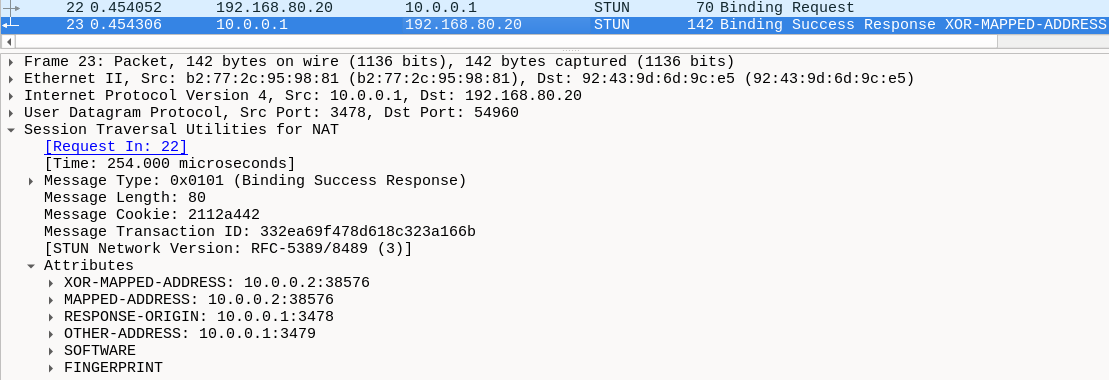
\includegraphics[width=1.0\textwidth]{fig/results/tests/stun_response_diff_mapping.png}
    \caption{Descoberta do endpoint público do gateway A no cenário
    com remapeamento.}
    \label{fig:result_stun_remap}
\end{figure}

Após a troca de candidatos, a WAN do roteador A registra um Binding Request destinado a \texttt{10.0.0.3:64027}, com \texttt{USERNAME}, \texttt{MESSAGE-INTEGRITY} e \texttt{USE-CANDIDATE}, seguido de uma resposta de sucesso. O destino é o endpoint público do gateway B, cuja porta local 47643 foi traduzida para 64027. A seleção registrada pela \texttt{libnice} corresponde ao par
\texttt{10.0.0.2:38576} e \texttt{10.0.0.3:64027}. Essa sequência vincula a descoberta, a nomeação do par e a comunicação posterior a portas públicas diferentes das portas locais. Assim, nesse cenário, o transporte ICE remove a dependência do ``mapeamento espelhado'' presente na referência sem ICE.

No caso C11 (QUIC/ICE direto), a captura permite acompanhar também a passagem da negociação ICE para o estabelecimento QUIC. Ao analisar a Figura \ref{fig:result_ice_quic_direct}, os quadros
26 e 27 contêm a nomeação e a resposta STUN, e descrevem as próprias etapas de UDP \textit{hole punching} a partir dos \textit{connectivity checks}. Posteriormente, o quadro 59 apresenta um datagrama UDP de 1200 bytes iniciado por um pacote QUIC Initial. A sequência inclui Retry e pacotes Handshake entre \texttt{10.0.0.2:49381} e \texttt{10.0.0.3:38368}. Esses são os \textit{endpoints} do par reflexivo selecionado nos \textit{logs}. Entre os \textit{checks} e o Initial aparecem os pequenos datagramas de controle do procedimento de descoberta mantido pelo \textit{backend} QUIC. A captura, portanto, permite distinguir a preparação do caminho do \textit{handshake} QUIC descrito na implementação.

% FIGURA 2: network_quic_ice_tcp/pcap/router-a/wan.pcap.
% Filtro: (frame.number >= 25 && frame.number <= 32) ||
%         (frame.number >= 59 && frame.number <= 73)
% Dois painéis: checks STUN (selecionar 26) e handshake (selecionar 59).
% Mostrar No., Time, Source, Destination, Protocol, Info e portas UDP.
% Sem chaves da sessão, não usar a imagem para afirmar validação de
% certificado nem para mostrar o conteúdo cifrado dos pacotes Handshake.
\begin{figure}[htbp]
    \centering
    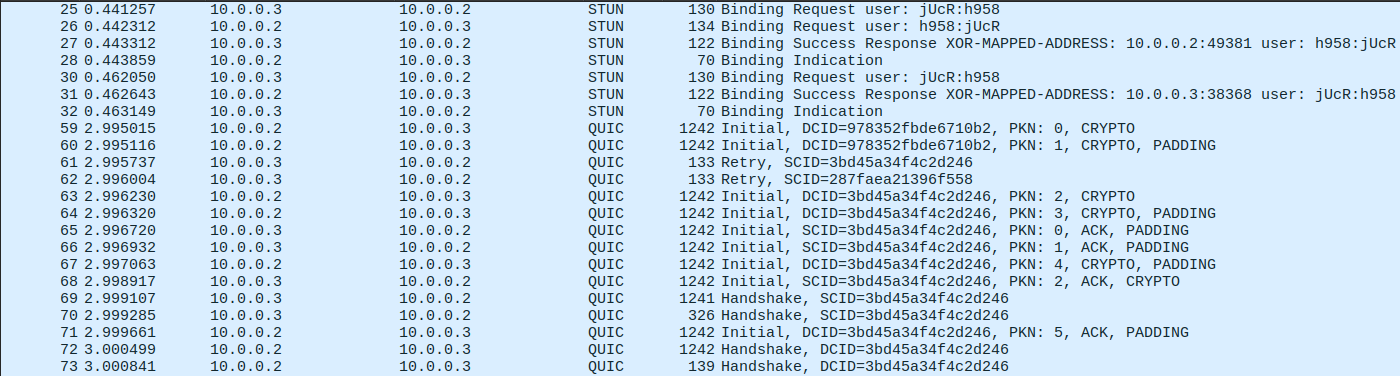
\includegraphics[width=1.0\textwidth]{fig/results/tests/cc_and_quic_handshake.png}
    \caption{Estabelecimento QUIC sobre o caminho ICE direto.}
    \label{fig:result_ice_quic_direct}
\end{figure}

A Tabela~\ref{tab:functional_paths} sintetiza as seleções da suíte regular (C1--C12). Nos quatro casos ICE diretos (C6, C7, C9 e C11), os dois candidatos foram identificados como reflexivos de servidor. Nos três casos com TURN obrigatório (C8, C10 e C12), ambos os candidatos eram relay.

\begin{table}[htbp]
    \centering
    \small
    \caption{Caminhos observados nos testes de estabelecimento.}
    \label{tab:functional_paths}
    \begin{tabular}{@{}p{0.43\textwidth}p{\dimexpr0.57\textwidth-2\tabcolsep\relax}@{}}
        \toprule
        \textbf{Cenários} & \textbf{Caminho observado} \\
        \midrule
        C1--C5: Chownat e QUIC sem ICE & UDP direto, com endpoints configurados previamente. \\
        C6 e C7: transporte ICE direto e com remapeamento & Par reflexivo de servidor/reflexivo de servidor. \\
        C9 e C11: Chownat/ICE e QUIC/ICE diretos & Par reflexivo de servidor/reflexivo de servidor. \\
        C8, C10 e C12: transporte ICE, Chownat/ICE e QUIC/ICE via TURN & Par relay/relay, com allocations no servidor. \\
        \bottomrule
    \end{tabular}
\end{table}

O uso de TURN altera o caminho de dados, além da seleção informada pela biblioteca. No caso C12 (QUIC/ICE/TURN), a resposta \textit{Allocate} informa \texttt{10.0.0.1:49191} como endereço de \textit{relay} do \textit{gateway} A. O ChannelBind associa o canal \texttt{0x4000} ao \textit{relay} remoto \texttt{10.0.0.1:49172}; em seguida, a WAN registra mensagens ChannelData entre \texttt{10.0.0.2:47158} e o servidor \texttt{10.0.0.1:3478}. No quadro 64, como visto na Figura \ref{fig:result_turn_data_path}, uma dessas mensagens contém 1200 \textit{bytes} de dados encapsulados, além do cabeçalho ChannelData de quatro \textit{bytes}. A captura evidencia, assim, o encapsulamento acrescentado pelo adaptador ICE sem alterar a interface utilizada pelo \textit{backend} QUIC (Figura~\ref{fig:openssl_quic_bio_update}).

\begin{figure}[htbp]
    \centering
    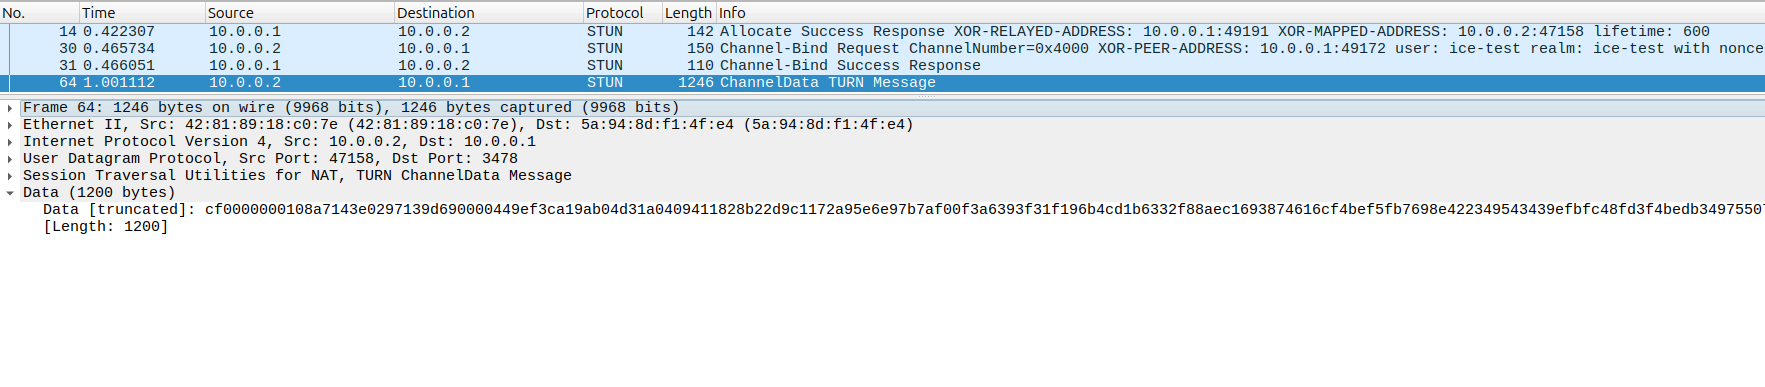
\includegraphics[width=1.0\textwidth]{fig/results/tests/turn_allocate_data_transfer.png}
    \caption{Caminho QUIC/ICE via TURN: \textit{allocation}, associação do canal
    ao relay remoto e transporte de dados por ChannelData.}
    \label{fig:result_turn_data_path}
\end{figure}

Os casos C8, C10, C12 e C13 utilizam \texttt{force\_relay} (opção que obriga a \texttt{libnice} a utilizar um servidor \textit{relay}). Demonstram o transporte pelo servidor quando esse caminho é imposto, mas não avaliam a transição automática de uma tentativa direta malsucedida para TURN.

\subsection{Transferência de dados e integração com aplicações TCP}
\label{sec:functional_data_transfer}

A verificação dos dados foi realizada nas interfaces entregues às aplicações, pois a conclusão do \textit{handshake} não demonstra que o túnel preserva o conteúdo transmitido. Nos seis casos curtos de túnel TCP (C3, C5 e C9--C12), o gerador enviou 16384 bytes e comparou a resposta do serviço \textit{echo} byte a byte.

O caso C11 (QUIC/ICE direto) ilustra a relação entre as duas conexões TCP locais e o transporte entre \textit{gateways}. No \textit{gateway} A, a aplicação se conecta à porta 44444, e o quadro 86 da captura de \textit{loopback} (Figura \ref{fig:result_tcp_application}(a)) contém os 16384 bytes entregues ao túnel. No \textit{gateway} B (Figura \ref{fig:result_tcp_application}(b)), a implementação abre outra conexão TCP com o serviço \textit{echo} na porta 1234. Nessa segunda conexão, o primeiro segmento de dados observado contém 1024 bytes, e os demais completam a mesma sequência de aplicação. As fronteiras dos segmentos são diferentes, enquanto o conteúdo entregue ao serviço é preservado.

\begin{figure}[htbp]
    \centering

    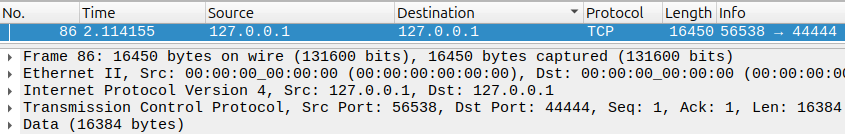
\includegraphics[width=0.90\linewidth]{fig/results/tests/tcp_local_payload.png}
    \\ Gateway A — envio dos dados TCP
    
    \par\medskip

    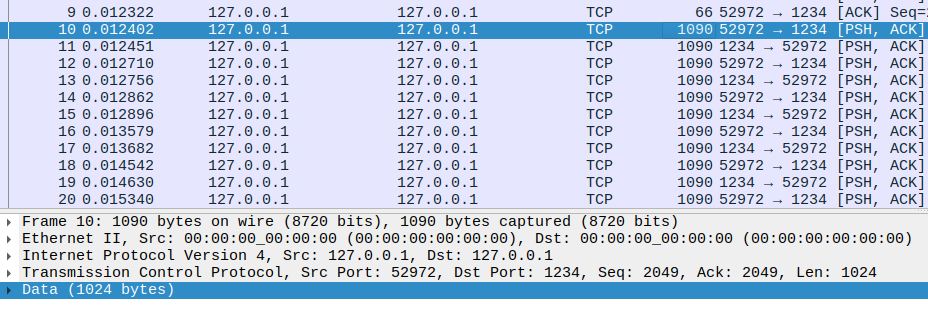
\includegraphics[width=0.90\linewidth]{fig/results/tests/tcp_remote_payload.png}
    \\ Gateway B — recepção dos dados TCP

    \caption{Integração com aplicações TCP no cenário QUIC/ICE direto.}
    \label{fig:result_tcp_application}
\end{figure}

Para conferir o conteúdo além do recorte visual, os dados foram reconstruídos a partir dos números de sequência TCP dessas duas capturas. Os quatro fluxos unidirecionais, correspondentes à ida e à volta em cada gateway, continham exatamente 16384 bytes, sem lacunas, e eram idênticos ao payload de referência. Isso relaciona os bytes enviados pela aplicação aos recebidos pelo serviço remoto e aos devolvidos na resposta. A evidência sustenta o tunelamento de dados descrito na Figura~\ref{fig:udp_conn_tcp_tunneling_diagram}: os segmentos TCP pertencem às conexões locais, e os dados atravessam a rede externa pelo transporte QUIC selecionado.

\begin{table}[htbp]
    \centering
    \small
    \caption{Resultados das verificações de conteúdo e entrega às aplicações.}
    \label{tab:functional_transfer}
    \begin{tabular}{@{}p{0.36\textwidth}p{\dimexpr0.64\textwidth-2\tabcolsep\relax}@{}}
        \toprule
        \textbf{Grupo de testes} & \textbf{Resultado observado} \\
        \midrule
        C1 e C4: Chownat e QUIC sem túnel & Três rodadas de requisição/resposta com conteúdo e sequência conferidos por protocolo. \\
        C6--C8: transporte ICE direto, remapeado e via TURN & Mensagens recebidas nos dois sentidos com conteúdo e tamanho esperados. \\
        C3, C9 e C10: Chownat com túnel TCP & Echo de 16384 bytes íntegro nas variantes sem ICE, ICE direto e ICE/TURN. \\
        C5, C11 e C12: QUIC com túnel TCP & Echo de 16384 bytes íntegro nas variantes sem ICE, ICE direto e ICE/TURN. \\
        \bottomrule
    \end{tabular}
\end{table}

No caso C2, dedicado ao encerramento Chownat, foram verificadas 20 mensagens recebidas no cliente e 21 no servidor, seguidas do fechamento e da liberação da sessão. Indicando o correto funcionamento configurado baseado no limite de tentativas do Chownat descrito na Tabela \ref{tab} que são utilizados tanto para tentativas de início de conexão tanto para o limíte de pacotes de \textit{keep-alive} enviados até considerar que uma conexão foi finalizada.

Nas quatro integrações de túnel com ICE (C9--C12), os contadores dos peers também registraram 16384 bytes enviados e recebidos por extremo e um único evento de conexão estabelecida. O resultado simultâneo nas variantes direta e TURN indica que a escolha do caminho ficou encapsulada no transporte, mantendo a entrega esperada pelas aplicações TCP locais. Essa conclusão se refere às cargas e às condições de rede exercitadas nesta coleta.

\subsection{Manutenção e encerramento das conexões}
\label{sec:functional_maintenance_shutdown}

Uma execução curta pode concluir a transferência antes de ser necessário renovar os recursos TURN. Por isso, o caso C13 manteve a sessão QUIC/ICE/TURN durante 67 transferências, com intervalos de 10~s entre os blocos a partir do segundo envio. Cada peer confirmou 1097728 bytes enviados e recebidos, e o teste completo, incluindo preparação e encerramento, terminou em 663,81~s. Sua duração permitiu observar renovações durante a mesma sessão.

A captura do gateway A mostra novos pedidos CreatePermission aproximadamente aos 241 e 481~s, ambos respondidos com sucesso. Aos 540~s, aparecem um Refresh e um ChannelBind, também seguidos de respostas de sucesso; a resposta ao Refresh informa \texttt{LIFETIME=600}. A Tabela~\ref{tab:functional_lifecycle} situa essas transações na captura, e a Figura~\ref{fig:result_turn_renewals} reserva os recortes correspondentes. Os registros do servidor confirmam as mesmas operações para a sessão do outro gateway.

\begin{table}[htbp]
    \centering
    \small
    \caption{Transações de manutenção e remoção na captura do gateway A
    durante o caso C13. Tempos relativos ao início dessa captura.}
    \label{tab:functional_lifecycle}
    \begin{tabular}{@{}p{0.15\textwidth}p{0.24\textwidth}p{\dimexpr0.61\textwidth-4\tabcolsep\relax}@{}}
        \toprule
        \textbf{Tempo (s)} & \textbf{Quadros} & \textbf{Transação e resposta} \\
        \midrule
        241,29 & 1312--1313 & CreatePermission e resposta de sucesso. \\
        481,73 & 2456--2457 & Nova renovação de permissão e resposta de sucesso. \\
        540,54 & 2757--2760 & Refresh com resposta LIFETIME 600 e renovação ChannelBind. \\
        662,14 & 3371--3374 & Remoção com LIFETIME zero, erro 438, novo pedido e sucesso. \\
        \bottomrule
    \end{tabular}
\end{table}

\begin{figure}[htbp]
    \centering
    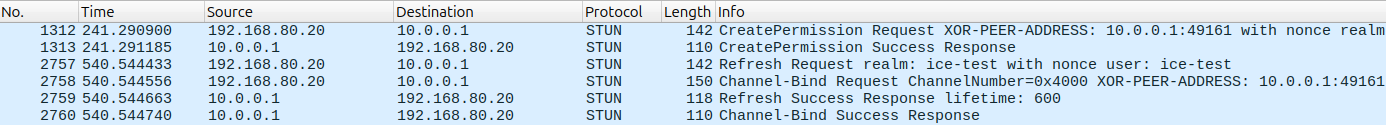
\includegraphics[width=1.0\linewidth]{fig/results/tests/renewals.png}
    \caption{Renovação dos recursos TURN durante a sessão QUIC/ICE.}
    \label{fig:result_turn_renewals}
\end{figure}

No encerramento do caso C13, o \textit{gateway} A solicita a remoção da allocation com \texttt{LIFETIME=0}, Como o \textit{nonce} utilizado já havia expirado, o servidor responde com erro 438 (\textit{Stale Nonce}) e fornece um novo \textit{nonce}. Em seguida, envia outro \textit{Refresh} com o \textit{nonce} fornecido nessa resposta e recebe sucesso com tempo de vida zero. Os dois pares de mensagens possuem identificadores de transação distintos: trata-se de um novo pedido autenticado, e não apenas da retransmissão do datagrama anterior.

\begin{figure}[htbp]
    \centering
    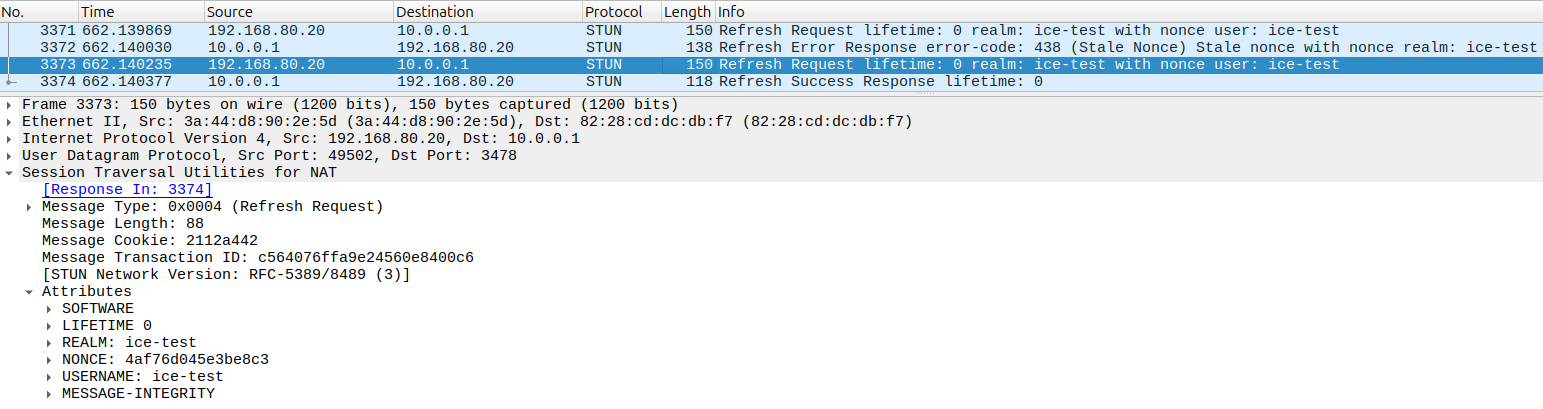
\includegraphics[width=1.0\linewidth]{fig/results/tests/turn_stale_nonce.png}
    \caption{Remoção da allocation TURN após expiração do nonce:
    tratamento do erro 438 e conclusão da nova transação de remoção.}
    \label{fig:result_turn_stale_nonce}
\end{figure}

Essa sequência permite verificar o efeito de uma correção aplicada à \texttt{libnice}. A correção faz a \texttt{libnice}, ao receber o erro 438 durante a remoção de uma allocation TURN, atualizar o nonce e repetir o pedido Refresh com \texttt{LIFETIME=0}. Antes, a biblioteca encerrava o procedimento localmente sem concluir a remoção no servidor. Com a correção, o recebimento do erro não encerrou o procedimento antes da remoção efetiva. O servidor registrou o erro 438 e a remoção com tempo de vida zero para os dois peers. Já o fechamento do túnel TCP é realizado localmente. O caso C13 demonstra a continuidade da transferência durante as renovações observadas e a conclusão do encerramento após erro 438.


\section{Avaliação em infraestrutura física controlada}
\subsection{Configuração dos equipamentos}
\subsection{Resultados e comparação com o ambiente PatchBay}

\cgk{adicionar esta implementação}



\section{Análise comparativa das abordagens de comunicação}
\label{sec:another_connection_approaches}

Para a análise lógica, foram propostos três cenários diferentes, contrapondo possíveis abordagens a serem utilizadas para a realização do mesmo tipo de comunicação: a abordagem P2P com ICE e QUIC desenvolvida neste trabalho; a abordagem mais comumente utilizada e aplicada na grande maioria dos dispositivos IoT, que segue um modelo de arquitetura do estilo cliente-servidor, a partir de um servidor especializado para a gerência das conexões; e uma abordagem P2P alternativa, utilizando comunicação TCP a partir de técnicas de TCP hole punching, como descritas na Seção~\ref{sec:tcp_hole_punching}.

\subsection{Comunicação P2P com ICE e QUIC}

Como base da análise lógica, pode-se utilizar a Figura~\ref{fig:non_centralized_quic_flow}, na qual é possível observar todo o processo lógico de conexão utilizando o ICE e, posteriormente, o protocolo QUIC para a conexão, e, após o estabelecimento desta, as trocas diretas entre cliente e servidor.

\begin{figure}[!ht]
    \centering
    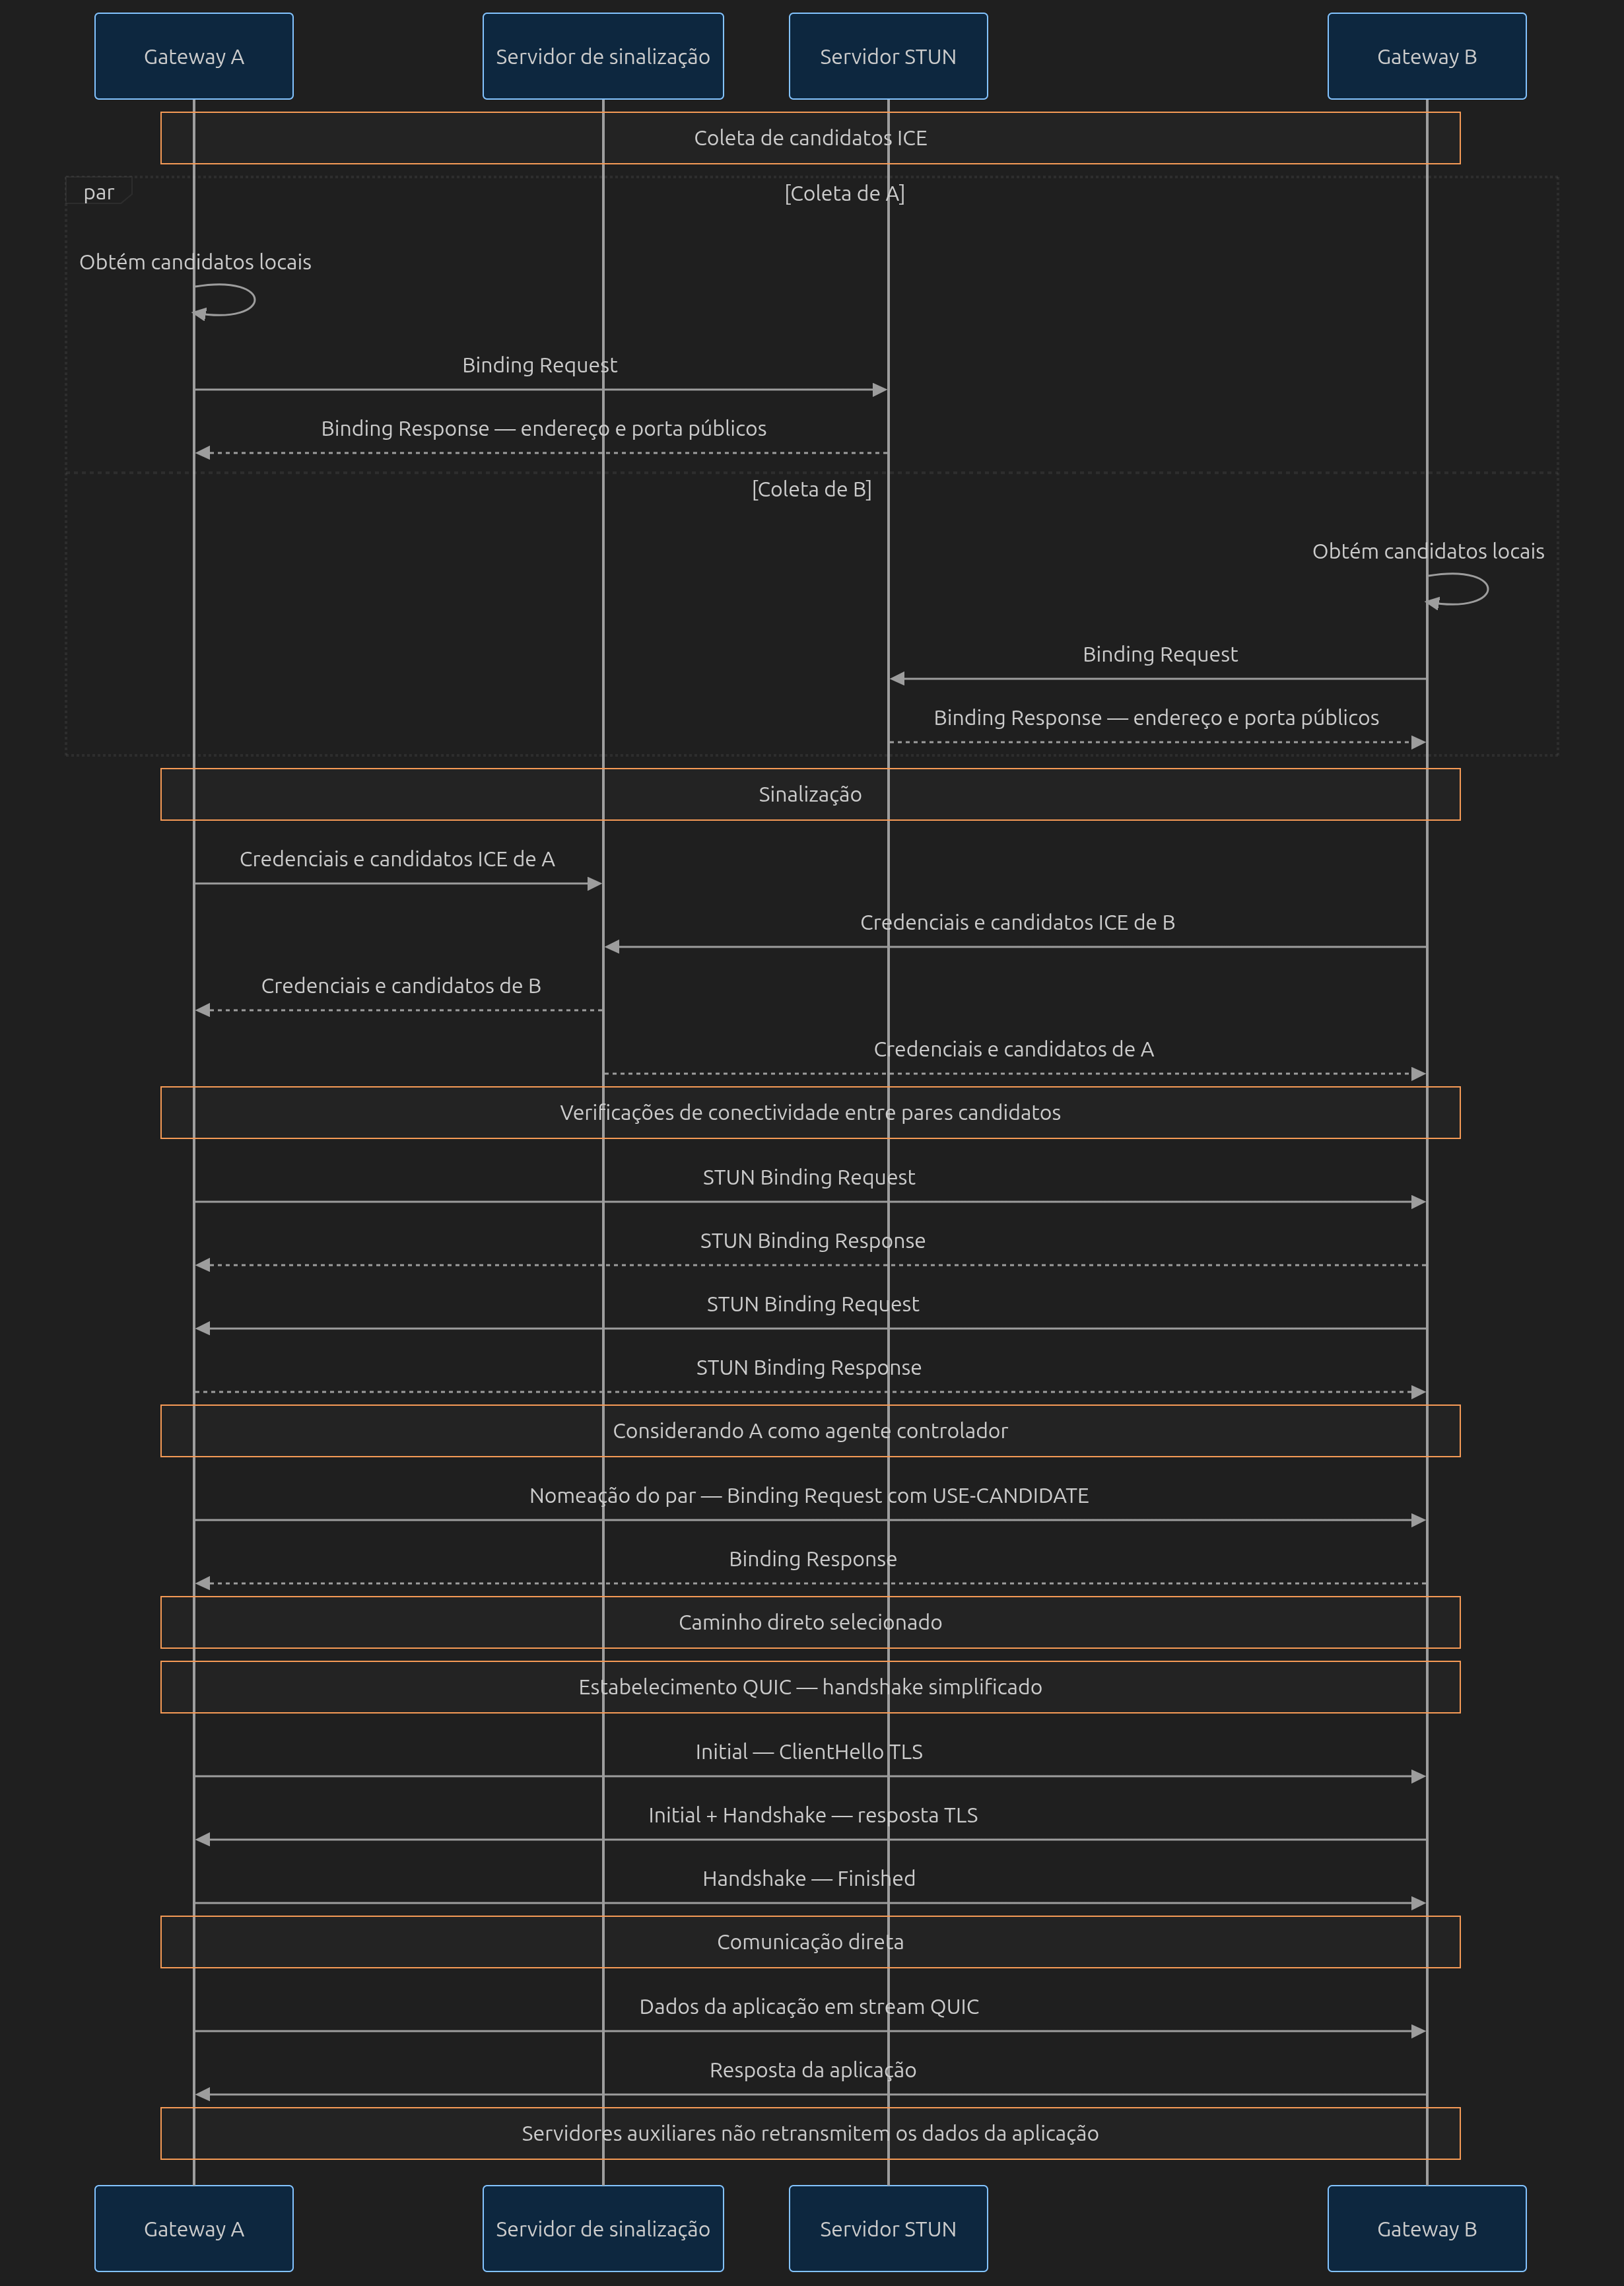
\includegraphics[width=0.8\textwidth]{fig/results/logic/flow_ice.png}
    \caption{Diagrama de tempo das etapas de comunicação utilizando o Protocolo ICE em união com o protocolo QUIC.}
    \label{fig:non_centralized_quic_flow}
\end{figure}

Importante lembrar que, ao utilizar um servidor TURN como \textit{fallback} -- isto é, caso a comunicação utilizando técnicas de \textit{hole punching} falhe --, ainda existiria um nível de indireção associado ao processo de estabelecimento, manutenção de conexão e troca de mensagens, acrescentando um custo adicional à comunicação.

\subsection{Comunicação com servidor intermediário especializado}

Ao se utilizar um servidor especializado, remove-se a obrigação do processamento em borda, o que aumenta a infraestrutura necessária. Para esta análise, o foco estará completamente nas etapas de conexão e no custo lógico de envio de mensagens entre os \textit{peers}; ainda assim, é importante manter em vista o custo infraestrutural envolvido, dado que a manutenção desse servidor também tem um custo. Nesta abordagem com um servidor intermediário, os dois \textit{peers} precisarão se conectar ao servidor, e, a partir disso, pacotes serão trocados entre eles. Suponha-se também um cenário ideal, no qual a comunicação entre \textit{peer} e servidor é feita por meio de um protocolo que já integra mecanismos de garantia de confidencialidade ao seu processo de conexão, como o QUIC -- caso fosse utilizado TCP/TLS, haveria ainda um custo adicional associado ao \textit{3-way handshake} do TLS.

A Figura~\ref{fig:centralized_server_quic_flow} descreve cada uma das etapas associadas a essa comunicação, sendo perceptível a diferença em relação ao fluxo descrito na Figura~\ref{fig:non_centralized_quic_flow}, principalmente quanto ao custo do uso do ICE nas etapas de estabelecimento da conexão da abordagem P2P. Em contrapartida, após o estabelecimento da conexão P2P, as mensagens são enviadas diretamente entre os pares, enquanto na abordagem com servidor especializado existe sempre um nível de indireção associado à retransmissão pelo servidor.

\begin{figure}[!ht]
    \centering
    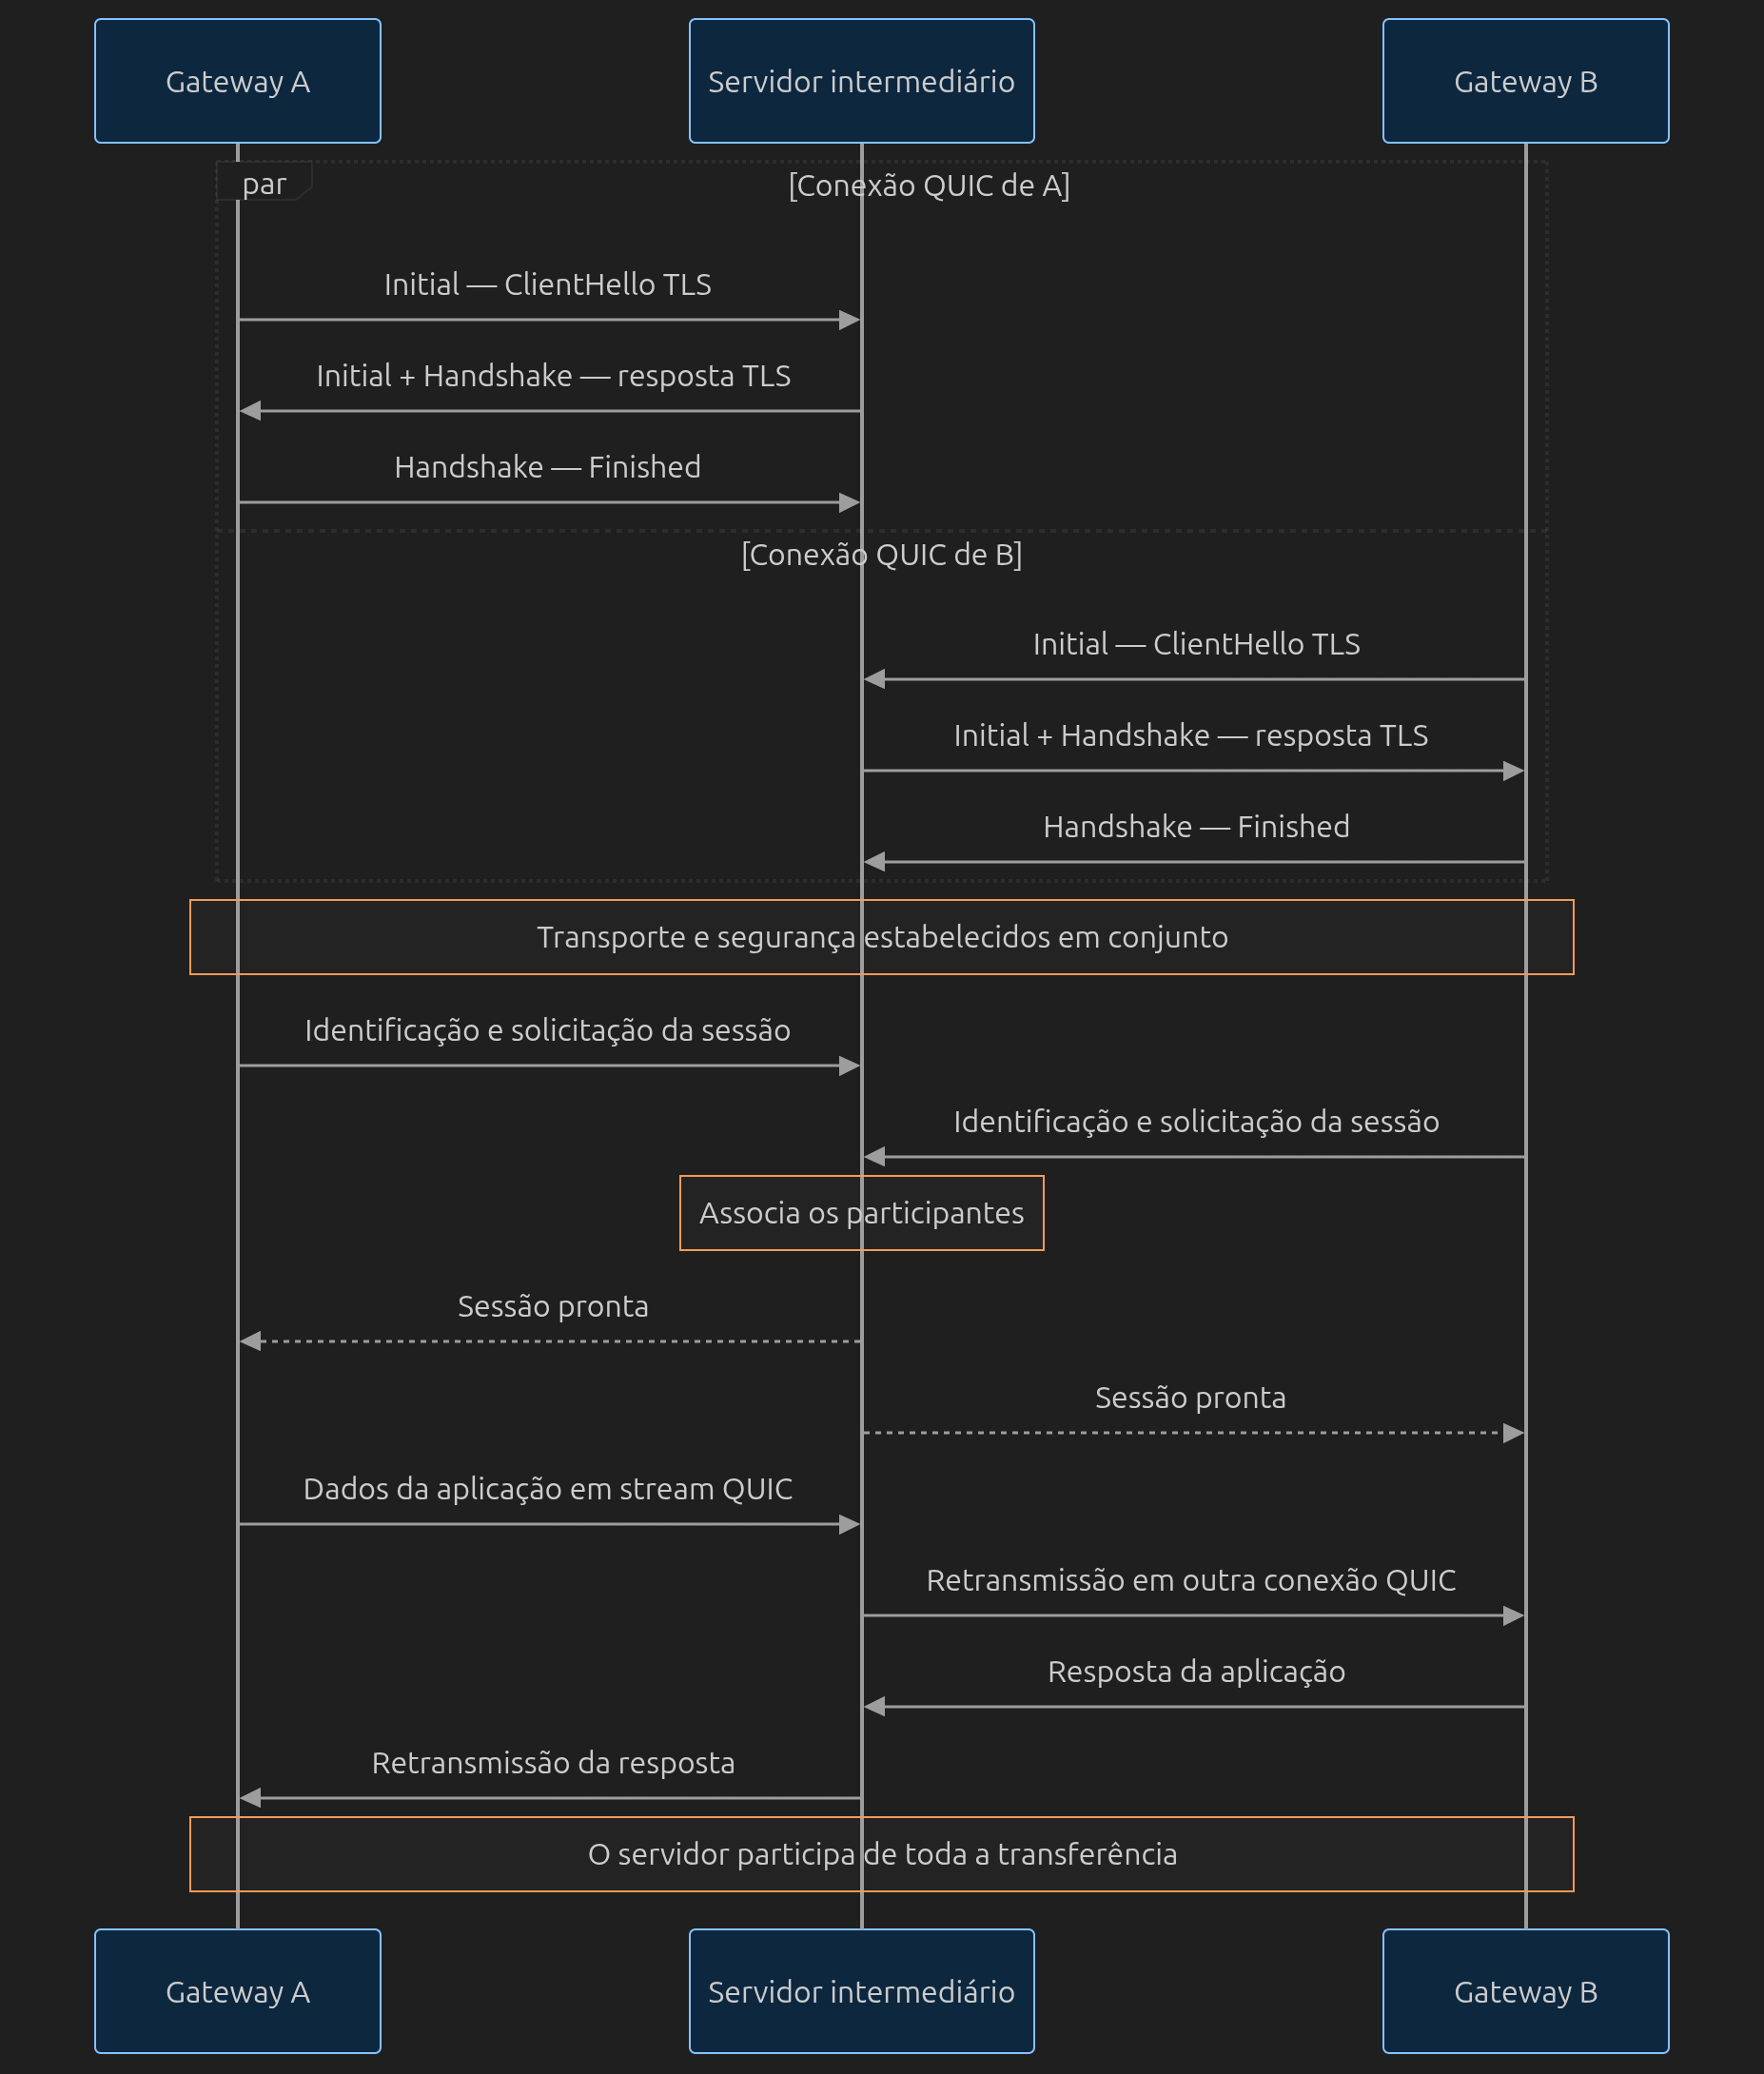
\includegraphics[width=0.8\textwidth]{fig/results/logic/centralized_server_quic_flow.png}
    \caption{Diagrama de tempo das etapas de comunicação utilizando um servidor especializado.}
    \label{fig:centralized_server_quic_flow}
\end{figure}

\subsection{Comunicação P2P com TCP hole punching}

Ao se utilizar TCP \textit{hole punching} sobre ICE, como descrito por \citep{rfc6544}, a comunicação entre os \textit{peers} ocorre de forma semelhante ao ICE para UDP descrito na Seção~\ref{sec:ice}. Entretanto, como o TCP não permite o envio de dados antes da existência de uma conexão estabelecida, é necessário realizar o TCP \textit{hole punching} de forma prévia à realização dos \textit{connectivity checks}; desta forma, os \textit{connectivity checks} mantêm como função principal a autenticação de cada par, e não mais a própria verificação de conectividade. Este fluxo pode ser visto na Figura~\ref{fig:non_centralized_ice_tcp_flow}.

\begin{figure}[!ht]
    \centering
    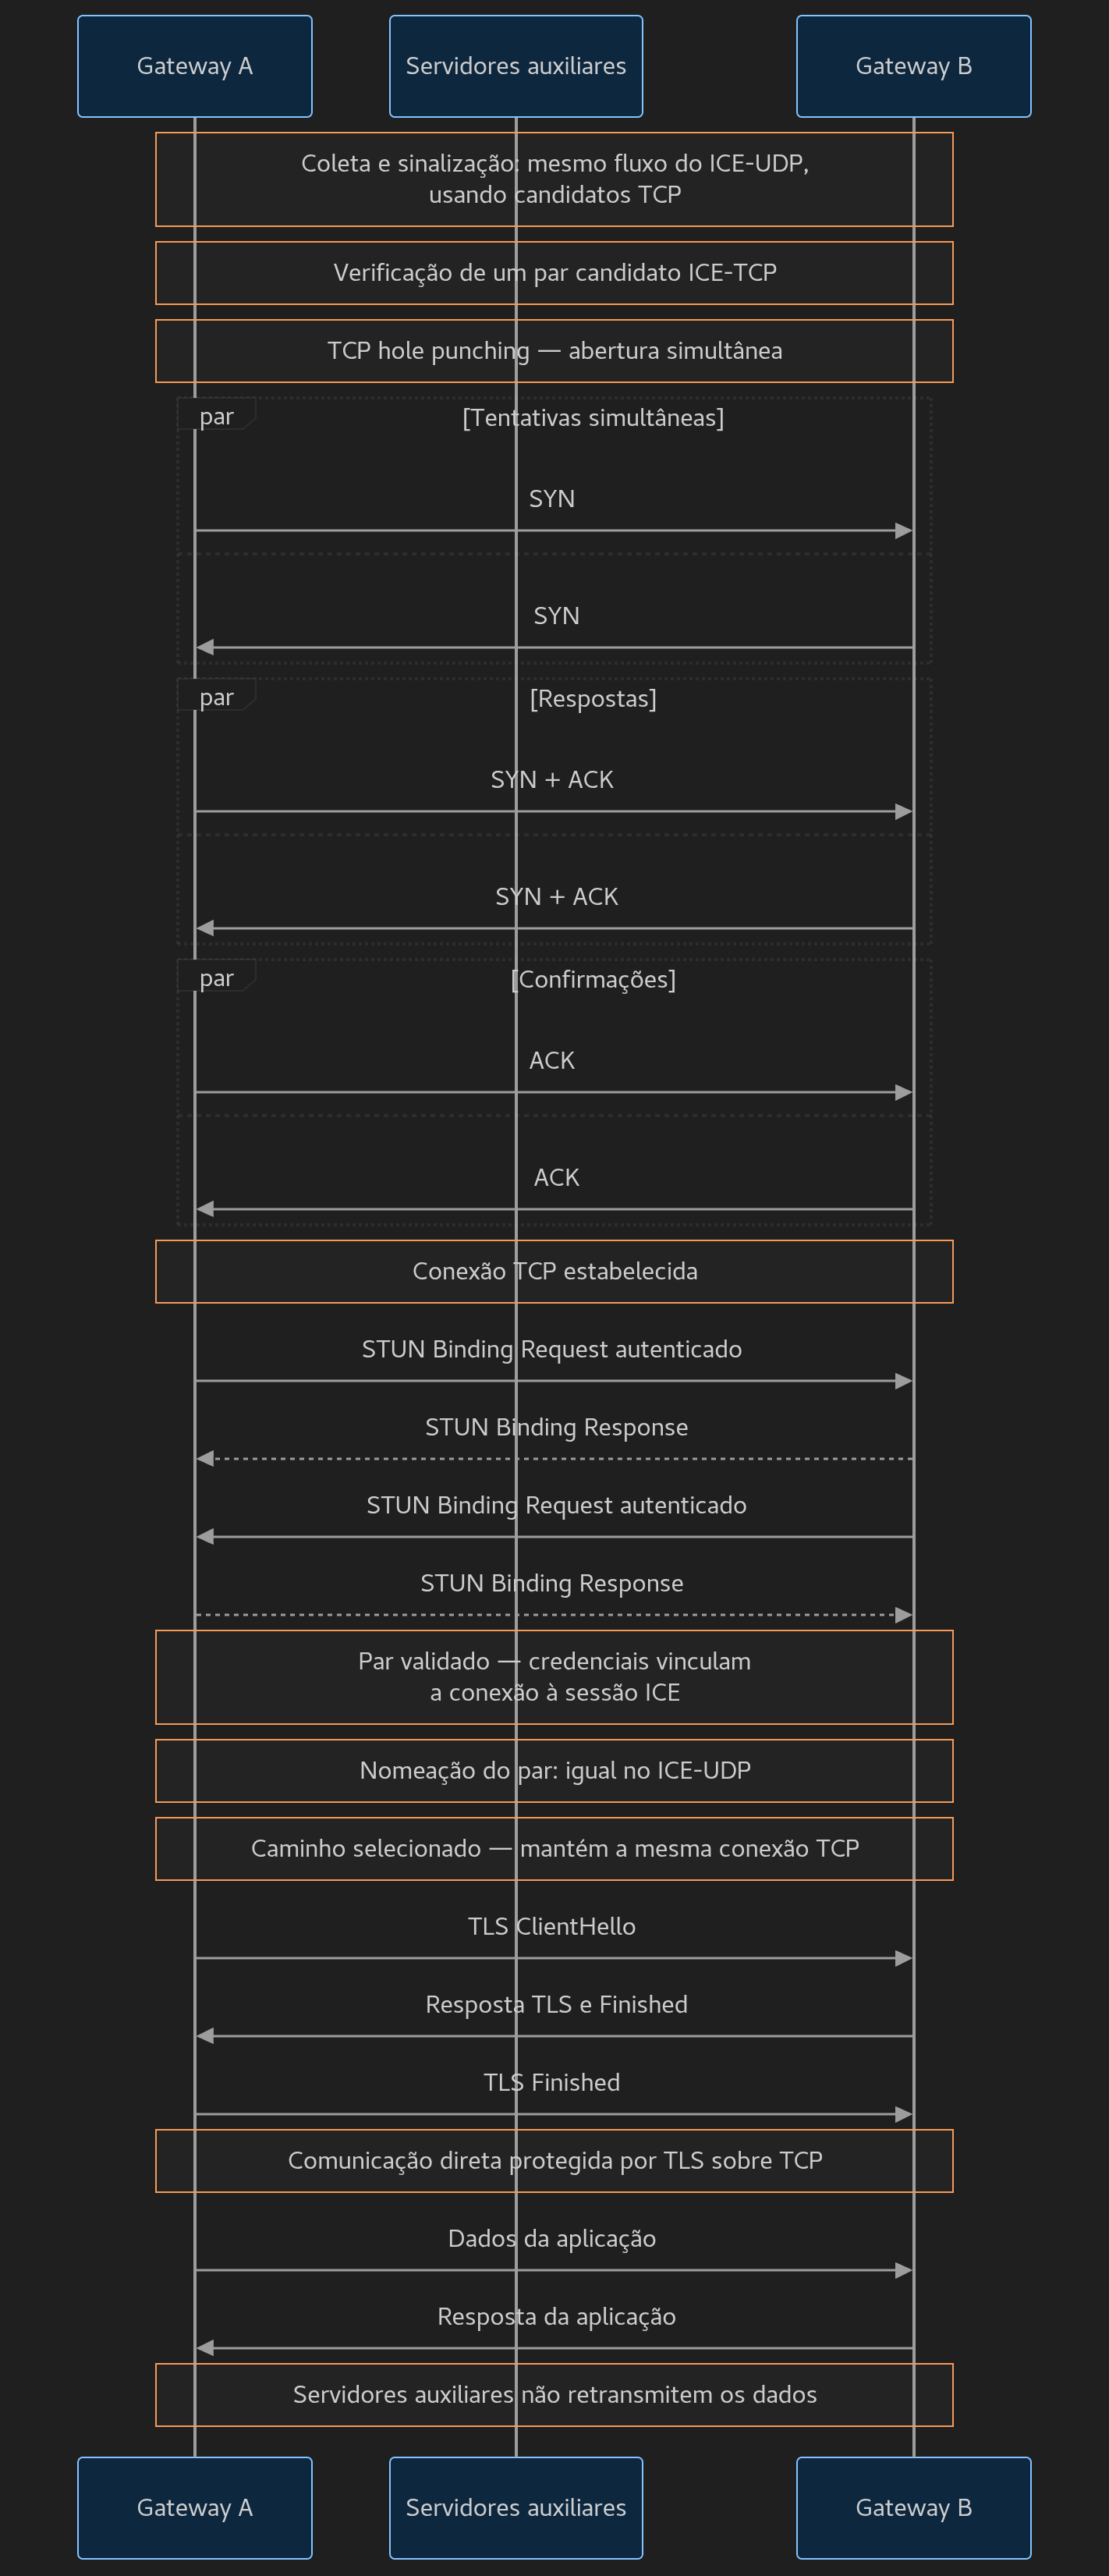
\includegraphics[width=0.5\textwidth]{fig/results/logic/flow_ice_tcp.png}
    \caption{Diagrama de tempo das etapas de comunicação utilizando ICE com TCP \textit{hole punching}.}
    \label{fig:non_centralized_ice_tcp_flow}
\end{figure}

\subsection{Comparação conceitual entre as abordagens}

Ao se utilizar uma conexão direta com o servidor, como proposto na Figura~\ref{fig:centralized_server_quic_flow}, o próprio servidor passa a ter acesso aos dados da aplicação, sem garantia de confidencialidade, dado que ele possui as chaves privadas tanto da conexão com o \textit{gateway}/\textit{peer} A quanto do \textit{gateway}/\textit{peer} B. Isto implica a necessidade de uma camada adicional de proteção dos dados de aplicação sobre essa comunicação, que não pode ser provida apenas pela camada de transporte. No caso do uso de um servidor TURN como \textit{fallback} da abordagem P2P, isto não ocorre: os dados enviados ao servidor são tunelados via TURN, e não por meio de uma conexão QUIC direta com o servidor, ou seja, a conexão QUIC permanece estabelecida de ponta a ponta entre os \textit{peers}, e o servidor TURN apenas retransmite os pacotes já cifrados.

Além disso, por se tratar de um servidor especializado, caso haja a queda deste, não há um servidor secundário que possa ser consultado para garantir a disponibilidade do serviço, o que não ocorre nas abordagens P2P, pois a solução é genérica e depende apenas de outro servidor que implemente o protocolo (não dependendo, por exemplo, de acesso direto a um banco de dados ou de alguma gerência específica).

Como visto por \citep{ford2005peer}, grande parte dos dispositivos NAT aceita técnicas de \textit{hole punching}, o que reduz a ocorrência da necessidade de uso de um servidor \textit{relay}/TURN nas abordagens P2P, tornando o cenário de indireção descrito como desvantagem da abordagem centralizada menos frequente na prática do que poderia parecer à primeira vista.

Ao utilizar técnicas de TCP \textit{hole punching}, é possível notar pela Figura~\ref{fig:non_centralized_ice_tcp_flow} que o estabelecimento da comunicação fica ainda mais lento: além da validação de candidatos, ainda é necessária a realização de uma dupla conexão TCP simultânea, adicionando mais dois \textit{3-way handshakes}. Além disso, a criptografia depende do TLS, que roda de forma separada do TCP, adicionando ainda outro \textit{handshake}.

Do ponto de vista operacional, as conexões TCP também podem ser consideradas mais frágeis por manterem metadados da conexão, como o número de sequência, expostos em texto claro, ao contrário do QUIC, que, como visto na Seção~\ref{sec:quic_header_protection}, protege criptograficamente essas informações mesmo no cabeçalho dos pacotes. Além disso, como visto por \citep{ford2005peer}, o TCP hole punching tem aproximadamente 20\% menos chance de efetivamente estabelecer a conexão do que o próprio UDP hole punching, além de possuir grandes dependências de sincronização, descritas na Seção~\ref{sec:tcp_hole_punching}.
